%% If you have any problems using this template, please contact the author: %%
%% timhosgood@gmail.com %%

\documentclass{beamer}
\usepackage[utf8]{inputenc}
\usepackage{charter}
\usepackage{tikz}
\usepackage{graphicx}
\usepackage{amsmath}
\usepackage{amssymb}
\usepackage{algorithm}
\usepackage{algpseudocode}




%% Title slide formatting %%

\pgfdeclareimage[width=\paperwidth]{titlebackground}{images/title-slide-background.png}
\setbeamerfont{subtitle}{size=\tiny}
\setbeamertemplate{title page}{
    \begin{picture}(0,0)
        \put(-28.5,-163){%
            \pgfuseimage{titlebackground}
        }
        \put(0,-75){%
            \begin{minipage}[b][4.5cm][t]{0.5\textwidth}
                \color{white}
                \usebeamerfont{title}
                    {\inserttitle\\[0.9cm]}
                \usebeamerfont{subtitle}
                    {\insertauthor\par}
                    {\insertinstitute\\[0.3cm]}
                    {\insertdate}
            \end{minipage}
        }
    \end{picture}
}



%% General slide formatting %%

\definecolor{oxfordblue}{RGB}{4,30,66}

\pgfdeclareimage[width=0.9cm]{oxfordlogo}{images/oxford-logo.png}
\pgfdeclareimage[width=1cm]{mathslogo}{images/mathematics-logo.png}

\setbeamertemplate{headline}
{%
    \begin{picture}(0,0)
        \put(314,-50){%
            \pgfuseimage{oxfordlogo}
        }
        \put(20,-55){%
            \rule{320pt}{0.4pt}
        }
    \end{picture}
}

\setbeamertemplate{frametitle}
{%
    \begin{picture}(0,0)
        \put(-8,-10){%
            \normalsize\color{oxfordblue}\insertframetitle
        }
        \put(-7,-20){%
            \tiny\color{oxfordblue}\insertframesubtitle
        }
    \end{picture}
}

\setbeamertemplate{footline}
{%
    \begin{picture}(0,0)
        \put(20,30){%
            \rule{320pt}{0.4pt}
        }
        \put(20,14){%
            \pgfuseimage{mathslogo}
        }
        \put(100,14){%
            \color{oxfordblue}\insertshortdate
        }
        \put(160,14){%
            \color{oxfordblue}\insertshorttitle
        }
        \put(337,14){%
            \color{oxfordblue}\insertpagenumber
        }
    \end{picture}%
}



%% Information (author, title, etc.) %%

\title[Dynamic regret and online convex optimization]{Online Convex Optimization and Dynamic Regret}
\author%
{%
    \sc{Wonsuk Yang}\\
}
\institute%
{%
    \textit{University of Oxford}
}
\date[Mar 2022]{Part C Dissertation Presentation, March 2022} % short date for footer



%% Content of slides %%

\begin{document}
    \begin{frame}[plain]
        \titlepage
    \end{frame}
    % Slide 1
    \begin{frame}
        % what is the problem?
        \frametitle{Introduction}
        \framesubtitle{Online convex optimization, non-stationary environment, and dynamic regret}
        \begin{itemize}
            \item The topic of the dissertation is \textbf{dynamic} regret in online convex optimization problems:
            \begin{center}
                $Reg_{T}^{D}(\mathbf{u}) = \sum_{t=1}^{T} f_{t}(x_t) - \sum_{t=1}^{T} f_{t}(u_t)$
            \end{center}
            % dynamic regret is defined as sum of losses incurred by our algorithm minus the total loss against a comparator.
            \item Unlike \textbf{static} regret, dynamic regret is more flexible, and is more appropriate when dealing with non-stationary environment.
            % difference between the cumulative loss of the player and that of the best fixed decision in hindsight
            \item As always, we seek for an algorithm that has sub-linear regret bound. 
            % Or, an algorithm that has upper bound matching the lower bound
            % and only recently has the lower bound for general online algorithm has been known
            \item The main challenge is to find an algorithm with a regret bound that is independent of both loss functions and comparator sequence (i.e. not problem specific).
            % The main goal of online convex optimization (OCO) is to find an algorithm that achieves sub-linear (static) \textbf{regret}: 
            % This means that the average loss goes to 0 as we run the algorithm infinitely long time.  
            % In practice, we run our algorithm against a non-stationary environment, so static regret is inappropriate in this setting.
            % That is, we compare the loss incurred by a sequence of actions selected by our algorithm against a comparator sequence.
            % One thing to note is that this is a generalization of static regret, since we can take the comparator sequence as a constant sequence $u_t = argmin_{x \in F} \sum_{t=1}^{T} f_t(x)$
            % As always, we seek for 
        \end{itemize}
    \end{frame}
    % Slide 2
    \begin{frame}
        \frametitle{Literature Review}
        \framesubtitle{Online convex optimization, non-stationary environment, and dynamic regret}
        \begin{itemize}
            \item There have been various works (Zinkevich, 2003; Cesa-Bianchi \& Lugosi, 2006; Hazan et al., 2006; Duchi et al., 2010, Shalev-Shwartz, 2012) on online algorithms that guarantee sub-linear bound on static regret.
            % Assuming convexity, we get O(sqrt(T)); assuming further regularity (for instance, strong convexity), we obtain better bounds (e.g. O(log(T)))
            \item Zinkevich (2003) first introduced dynamic regret, and showed OGD with constant step size achieves $O(\sqrt{T}(1+P_T))$ upper bound on dynamic regret.
            % P_T is path length, sum of norm of difference between consecutive elements of the comparator sequence. 
            \item Zhang et al. (2018) and Zhao et al. (2020) established the lower bound, and introduced algorithms whose regret upper bounds match the lower bounds for OCO and BCO (two point) respectively.
        \end{itemize}    
    \end{frame}
    % \begin{frame}
    %     \frametitle{Literature Review}
    %     \framesubtitle{Online convex optimization, non-stationary environment, and dynamic regret}
    %     \begin{center}
    %         \begingroup
    %             \setlength{\tabcolsep}{10pt}
    %             \renewcommand{\arraystretch}{1.2}
    %             \begin{tabular}{c c c c}
    %                 \hline
    %                 Complexity Measure & Loss function & Dynamic Regret & Reference \\
    %                 \hline \hline
    %                 Path-length & Convex & $O(\sqrt{T(1 + P_T)})$ & Zinkevich, 2003 \\
    %                 Path-length & Strongly Convex + Smooth & $O(P_T)$ & Mokhtari, 2006 \\
    %                 Path-length & Convex & $O(\sqrt{T(1 + P_T)}$ & Zhang et al., 2018 \\
    %                 Functional Variation & Convex & $O(T^{2/3}V_T^{1/3})$ & Besbes et al., 2015 
    %             \end{tabular}
    %         \endgroup
    %     \end{center}
    % \end{frame}
    % Slide 3
    \begin{frame}
        \frametitle{Algorithm}
        \framesubtitle{Reference: Zhang et al., Adaptive Online Learning in Dynamic Environments, 2018}
        \begin{itemize}
            \item Under some minor assumptions, it is known that for any online algorithm, there is a sequence of loss functions and comparators such that $Reg_T^{D}(\mathbf{u}) = \Omega(\sqrt{T(1 + P_T)})$.
            % assumptions: 
            % 1) loss functions are bounded and its gradient bounded globally and uniformly 
            % 2) feasible set is bounded
            % Therefore, our baseline (OGD with constant step size) is far from optimal
            \item Key observation: If the path length is known a priori, then we obtain an optimal step size $\eta = O(\sqrt{(1 + P_T)/T})$ where OGD attains regret bound $O(\sqrt{T(1+P_T)})$.
            % In sum we have a delimma -- On one hand, we want the regret bound to hold for any sequence of comparators, but on the other hand, to get a tighter bound, we need to tune the step size for a specific path-length.
            \item Hence, we run \textit{multiple OGD with different step sizes}, and combine them via \textit{exponentially weighted average forecaster algorithm} to select optimal action at each step (ADER).
            % ADER Adaptive Learning for Dynamic Regret
            % prediction with expert advice
            % What does exponentially weighted average forecaster algorithm do? 
            % Explain HERE...
            \item We can select specific set of step sizes so that the algorithm attains $O(\sqrt{T(1 + P_T)})$ regret bound.
            % only depends on the bounds on feasible set and the global l2 bound on the gradient.
            % independently of given comparator sequence and loss functions!!! 
        \end{itemize}    
    \end{frame}
    % Slide 4
    \begin{frame}
        \frametitle{Algorithm}
        \framesubtitle{Reference: Zhang et al., Adaptive Online Learning in Dynamic Environments, 2018}
        \begin{figure}
            \centering
            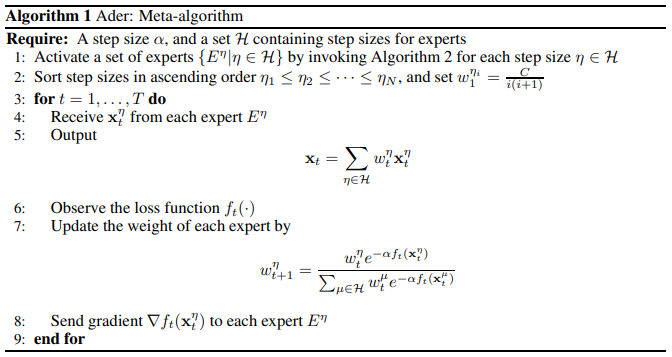
\includegraphics[scale=0.6]{images/ader-meta.PNG}
            \caption{Meta algorithm \\ (taken from Zhang et al.)}
            \label{fig:comb}
        \end{figure}
    \end{frame}
    % Slide 5
    \begin{frame}
        \frametitle{Algorithm}
        \framesubtitle{Reference: Zhao et al., Bandit Convex Optimization in Non-stationary Environments, 2020} 
        \begin{itemize}
            \item Similar method can be used for \textbf{bandit convex optimization problem}.
            % Here we are faced with additional challenge of not having access to the gradient of the function. We resolve this issue with gradient estimator.
            % In bandit convex optmization problem, we are allowed to query the value of function, and do not have access to gradients.
            \item We replace gradients by gradient estimators (Agarwal et al., 2010), given as follows (two point feedback),
            \begin{center}
                $\Tilde{g}_{t} = \frac{d}{2\delta}(f_{t}(x_t + \delta u_t) - f_{t}(x_t - \delta u_t))u_t$
                % for one point feedback, we use $\frac{d}{\delta}f_{t}(x_t + \delta u_t)u_t$
                % these happens to be an unbiased estimators of gradient (with u_t being random)
                % d is the dimension of the feasible set, \delta is a perturbation parameter
                % u_t is sampled from unit sphere 
            \end{center}
            This estimator is an unbiased estimator of the smoothed loss function $\hat{f}_{t}(x) = \frac{d}{\delta}\mathbb{E}[f(x + \delta u)u]$.
            % and this loss function is used to update the weights.
            \item For two point feedback model, the algorithm attains regret bound of order $O(\sqrt{T(1+P_T)})$, which matches the lower bound $\Omega(\sqrt{T(1+P_T)})$.
            % For one point feedback case, the algorithm attains upper bound $O(T^{3/4}(1+P_T)^{1/2})$.
        \end{itemize}    
    \end{frame}
    % Slide 6
    \begin{frame}
        \frametitle{Conclusion and Future Work}
        \framesubtitle{Online convex optimization, non-stationary environment, and dynamic regret}
        \begin{itemize}
            \item We introduce dynamic regret and motivate its necessity. 
            % Regularity assumptions related to the comparator sequence.
            \item We establish $\Omega(\sqrt{T(1+P_T)})$ lower bound on dynamic regret for any online algorithm. 
            \item We introduce ADER, an online algorithm that achieves $O(\sqrt{T(1+P_T)})$ upper bound on dynamic regret. Its variant for BCO achieves same upper bound in case of two-point feedback. 
            \item We modify ADER to get a tighter bound when the loss functions are assumed to be strongly convex and/or smooth.
        \end{itemize}    
    \end{frame}
    % Slide 6
    \begin{frame}
        \frametitle{Main Reference}
        \framesubtitle{Online convex optimization, non-stationary environment, and dynamic regret}
        \begin{itemize}
            \item Hazan, Elad. “Introduction to Online Convex Optimization.” Found. Trends Optim (2016).
            \item Yang, Tianbao et al. “Tracking Slowly Moving Clairvoyant: Optimal Dynamic Regret of Online Learning with True and Noisy Gradient.” ICML (2016).
            \item Zhang, Lijun et al. “Adaptive Online Learning in Dynamic Environments.” NeurIPS (2018).
            \item Zhao, Peng et al. “Bandit Convex Optimization in Non-stationary Environments.” AISTATS (2020).
        \end{itemize}    
    \end{frame}
\end{document}